\newpage
\clearpage
\section{Segmentação de Imagens}
\label{segment}

A segmentação de imagens é uma área que se enquadra nas disciplinas de visão computacional e processamento digital de imagens, visando principalmente a distinção de áreas ou propriedades específicas em uma imagem \citep{Haralick1985, Yuheng2017, Ghosh2019}. Este processo possibilita análises mais precisas ou a separação de áreas de interesse de acordo com os objetivos da análise.

A segmentação de imagens desempenha um papel fundamental em várias aplicações, incluindo reconhecimento facial \citep{Yuheng2017}. Além disso, áreas como medicina, veículos autônomos, sensoriamento remoto e outras também se beneficiam significativamente dessas técnicas. Para ilustrar, as Figuras \ref{segment:fig:1.1} e \ref{segment:fig:1.2} representam segmentações faciais e médicas, respectivamente.

\begin{figure}[H]
   \caption{Exemplos de segmentações de imagens.}
   \centering
   \label{segment:fig:1}
    \begin{subfigure}[t]{0.6\textwidth}
        \centering
        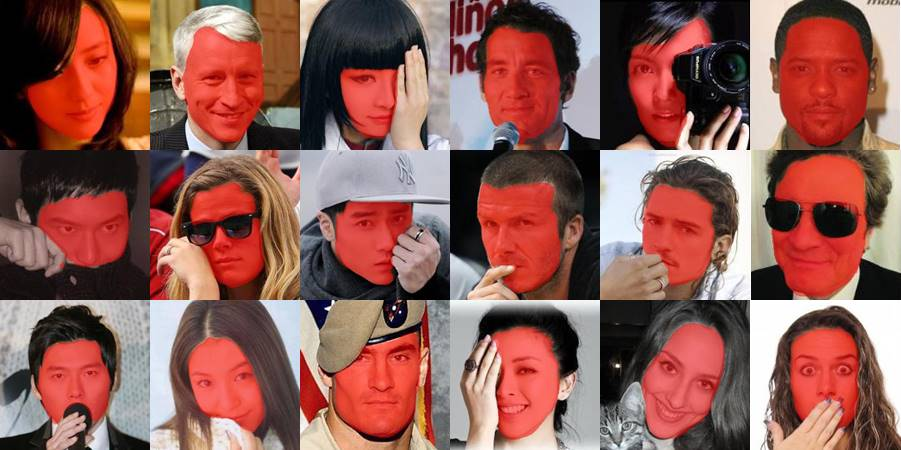
\includegraphics[width=1\linewidth]{recursos/imagens/image_seg/faces.png}
        \caption{Segmentação de imagens faciais.}
        \label{segment:fig:1.1}
    \end{subfigure}%
    ~ 

    \begin{subfigure}[t]{0.6\textwidth}
        \centering
        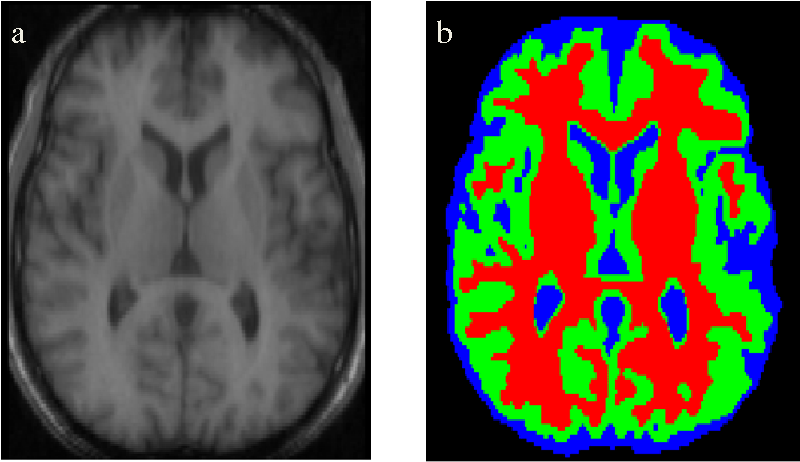
\includegraphics[width=1\linewidth]{recursos/imagens/image_seg/cerebro.png}
        \caption{Segmentação de imagem médica.}
        \label{segment:fig:1.2}
    \end{subfigure}%
    ~

    Fonte: \cite{Nirkin2018} e \cite{Withey2008}, respectivamente.
\end{figure}

Para demonstrar o funcionamento das segmentações de maneira matemática, consideramos um conjunto de imagens $I$ definido em um domínio $\Omega \subset \mathbb{R}^d$, onde $d \geq 2$. A imagem observada $I_0$ e os predicados lógicos $P_1, \ldots, P_n$ são utilizados para verificar $n$ afirmações expressas com base em características da imagem, como bordas, suavidade, textura ou cor. O predicado $P_k(A)$ pe verdadeiro se todos os pontos de $A \subseteq \Omega$ satisfizerem a $k$-ésica afirmação. Essa abordagem é inspirada em trabalhos anteriores, como mencionado por \cite{antonelli2022view}.

Por exemplo, para realizar uma segmentação de duas regiões em uma imagem em tons de cinza normalizada $I_0$, prdemos definir $n = 2$ afirmações simples. Essas afirmações estão relacionadas ao nível de cinza da intensidade da luz e são utilizadas para distinguir entre o plano de fundo e o primeiro plano, como demonstrado na Equação \ref{segment:eq:seg}.

\begin{equation}
\label{segment:eq:seg}
    P_1(A) = \{ I^\ast(x) < \alpha, \forall x \in A \}, \quad P_2(A) = \{ I^\ast(x) \geq \alpha, \forall x \in A \},
\end{equation}
em que $I^\ast(x)$ representa uma aproximação adequada de $I_0$ e $\alpha \in (0,1)$ é um valor escolhido de forma apropriada.

Compreendido o conceito de segmentação de imagens, esta área compreende uma ampla gama de técnicas, com a Seção \ref{segment:segment} abordando os métodos de segmentação tradicionais, que continuam sendo amplamente estudados e aplicados até os dias atuais.

\subsection{Métodos e Técnicas Tradicionais}
\label{segment:segment}

Quando se trata de segmentações, algumas técnicas são muito conhecidas e utilizadas, sendo que algumas são calculadas utilizando apenas convoluções matriciais simples \citep{Yuheng2017}.

Sendo assim, nas próximas seções algumas técnicas de segmentação serão discutidas, das quais pode-se citar as segmentações baseadas em regiões (Seção \ref{segment:region}), bordas  (Seção \ref{segment:limit}), baseada em grafos (Seção \ref{segment:graph}), \textit{watershed} (Seção \ref{segment:watershed}), \textit{liveware} (Seção \ref{segment:livewire}), \textit{superpixel} (Seção \ref{segment:superpixel}), agrupamentos (Seção \ref{segment:group}) e até mesmo as que fazem uso de redes neurais  (Seção \ref{segment:neural}) com a aplicação de alguns conceitos que foram comentados no Capítulo \ref{deep}.

\subsubsection{Segmentação Baseada em Regiões}
\label{segment:region}

Alguns tipos de segmentação comumente trabalham com os valores dos \textit{pixels}, de modo que seja possível segregar áreas e regiões de interesse de regiões que não são possuem relevância. Dentre as diversas técnicas, vale destacar a técnica de \textit{Threshold Segmentation}, ou em português, segmentação limiar, a qual é desenvolvida e aplicada em diversos trabalhos \citep{Yanowitz1989}.

De um modo geral, a segmentação por meio da determinação de um limiar acontece em imagens que utilizam a escala de cinza ou algum sistema de cor que possua um canal voltado para intensidade, como o sistema HSV \citep{schneider2003experimentos}, visto que quando no sistema correto, há a determinação de um valor entre o fundo e a área de interesse da imagem. Dessa forma, os \textit{pixels} acima do valor médio determinado são categorizados como área de intensidade e os inferiores são categorizados como fundo \citep{pedrini2008analise}, como é possível observar na Equação \ref{segment:eq:1}, em que $T$ representa o limiar determinado, $f(x,y)$ é um \textit{pixel} da imagem $f$ e $g(x,y)$ é este \textit{pixel} limiarizado:

\begin{equation}
\label{segment:eq:1}
    g(x,y) = \begin{cases}
        0,& se \; f(x,y) \leq T \\
        1,& se \; f(x,y) > T
    \end{cases}.
\end{equation}

Sobre \textit{threshold segmentation}, vale citar que há uma série de técnicas para determinar o valor de limiarização como é trabalhado por \cite{Atta2018ImageTechniques}, mas habitualmente utiliza-se da média \citep{Atta2018ImageTechniques, Yanowitz1989, Yuheng2017} ou de técnicas adaptativas que são citadas em trabalhos, como \cite{Yanowitz1989}, mas que ganham repercussões abrangentes e é evidenciada na técnica Otsu \citep{Otsu1979}, principalmente quando se trata de segmentações com um limiar global como demonstra o histograma na Figura \ref{segment:fig:2.1} e o exemplo prático na Figura  \ref{segment:fig:3.3}. Todavia, quando as regiões de interesse estão divididas, faz-se necessário a divisão de limiares locais, como pode ser observado no histograma da Figura \ref{segment:fig:2.2}, Equação \ref{segment:eq:2} ou na Figura \ref{segment:fig:3.4}:

\begin{equation}
\label{segment:eq:2}
    g(x,y) = \begin{cases}
        v1, & se \; f(x,y) \leq T \\ 
        v2, & se \; T_1 < f(x,y) \leq T_2 \\
        v3, & se \; f(x,y) > T_2
    \end{cases}.
\end{equation}

\begin{figure}[H]
   \caption{Histogramas de limiarizações.}
   \centering
   \label{segment:fig:2}
    \begin{subfigure}[t]{0.45\textwidth}
        \centering
        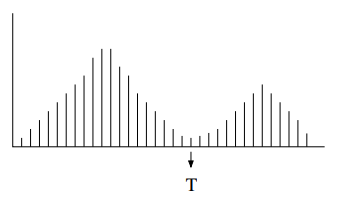
\includegraphics[width=1\linewidth]{recursos/imagens/image_seg/limi_glob.png}
        \caption{Histograma de limiarização global.}
        \label{segment:fig:2.1}
    \end{subfigure}%
    ~ 
    \begin{subfigure}[t]{0.45\textwidth}
        \centering
        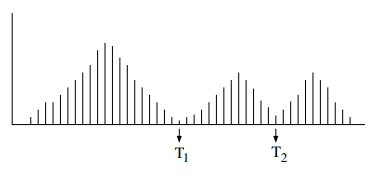
\includegraphics[width=1\linewidth]{recursos/imagens/image_seg/limi_local.png}
        \caption{Histograma de limiarização local.}
        \label{segment:fig:2.2}
    \end{subfigure}%

    Fonte: \cite{pedrini2008analise}.
\end{figure}

\begin{figure}[H]
   \caption{Limiarizações.}
   \centering
   \label{segment:fig:3}
    \begin{subfigure}[t]{0.45\textwidth}
        \centering
        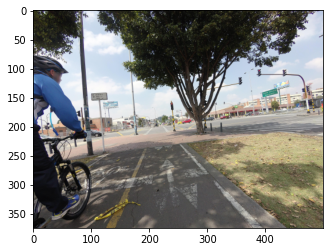
\includegraphics[width=1\linewidth]{recursos/imagens/image_seg/mapi.png}
        \caption{Imagem original.}
        \label{segment:fig:3.1}
    \end{subfigure}%
    ~ 
    \begin{subfigure}[t]{0.45\textwidth}
        \centering
        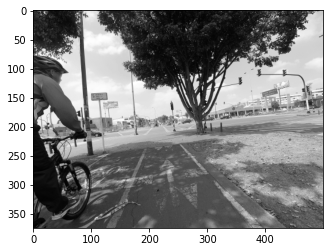
\includegraphics[width=1\linewidth]{recursos/imagens/image_seg/gray_mapi.png}
        \caption{Imagem em escala de cinza.}
        \label{segment:fig:3.2}
    \end{subfigure}%
    ~ 
    
    \begin{subfigure}[t]{0.45\textwidth}
        \centering
        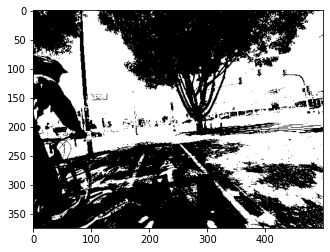
\includegraphics[width=1\linewidth]{recursos/imagens/image_seg/bw_mapi.png}
        \caption{Imagem limiarizada globalmente.}
        \label{segment:fig:3.3}
    \end{subfigure}
    ~
    \begin{subfigure}[t]{0.45\textwidth}
        \centering
        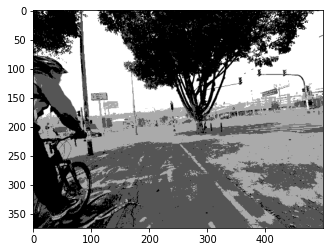
\includegraphics[width=1\linewidth]{recursos/imagens/image_seg/local_mapi.png}
        \caption{Imagem limiarizada localmente.}
        \label{segment:fig:3.4}
    \end{subfigure}

    Fonte: retirado e adaptado de \cite{Neuhold2017_ICCV}.
\end{figure}

Por fim, no contexto da segmentação baseada em regiões, destaca-se a técnica de crescimento de regiões, também conhecida como \textit{Region Growing}. Essa abordagem consiste em definir um limiar e distribuir sementes na imagem, de forma que os \textit{pixels} vizinhos sejam incorporados à região se as diferenças entre eles e as sementes forem inferiores ao limiar estabelecido. O efeito desse procedimento pode ser visualizado na Figura \ref{segment:fig:4} ou representado matematicamente pela Equação \ref{segment:eq:3}, onde $P(R)$ é o predicado da região, $f(r,s)$ é o \textit{pixel} semente, e $f(x,y)$ representa um \textit{pixel} vizinho ao da semente na vizinhança-8:

\begin{equation}
\label{segment:eq:3}
P(R) = \begin{cases}
    1, & se \; |f(x,y) - f(r,s)| \leq T \\
    0,      &  \text{caso contrário}
\end{cases}.
\end{equation}

Esta técnica é ilustrada na Figura \ref{segment:fig:4}, onde a Figura \ref{segment:fig:4.1} mostra a imagem original com os \textit{pixels} sementes em vermelho ($f(r,s)$). As Figuras \ref{segment:fig:4.2} e \ref{segment:fig:4.3} representam, respectivamente, o crescimento da região com limiares $T = 3$ e $T = 6$.

\begin{figure}[H]
   \caption{Ilustração do crescimento de região.}
   \centering
   \label{segment:fig:4}
    \begin{subfigure}[t]{0.45\textwidth}
        \centering
        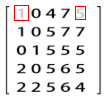
\includegraphics[height=1.5in]{recursos/imagens/image_seg/m1.png}
        \caption{Imagem original, sendo em vermelho os \textit{pixels} sementes ($f(r,s)$).}
        \label{segment:fig:4.1}
    \end{subfigure}
    ~ 
    \begin{subfigure}[t]{0.45\textwidth}
        \centering
        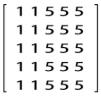
\includegraphics[height=1.5in]{recursos/imagens/image_seg/m2.png}
        \caption{Crescimento de região com $T = 3$.}
        \label{segment:fig:4.2}
    \end{subfigure}
    ~ 

    \begin{subfigure}[t]{0.45\textwidth}
        \centering
        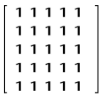
\includegraphics[height=1.5in]{recursos/imagens/image_seg/m3.png}
        \caption{Crescimento de região com $T = 6$.}
        \label{segment:fig:4.3}
    \end{subfigure}

    Fonte: retirado e adaptado de \cite{Yuheng2017}.
\end{figure}

Esta técnica é utilizada para agrupar \textit{pixels} que possuem similaridades entre si, formando regiões coesas na imagem.

Por fim, ainda sobre o aspecto de crescimento de região, salienta-se que é de extrema importância a determinação das sementes e do valor limiar \citep{Yuheng2017, pedrini2008analise}, além de ser necessário ter as condições para determinação de sistema de cores e canais semelhantes às de \textit{threshold segmentation}.


\subsubsection{Segmentação por Bordas}
\label{segment:limit}

Em meio às categorias de segmentação tradicional estão as segmentações por descontinuidade, com subcategorias de segmentação por pontos, retas, junções e, finalmente, por bordas \citep{pedrini2008analise}. Correntemente, é a partir dessas segmentações que são construídos alguns dos filtros convolucionais que foram explorados no Capítulo \ref{cnn}.

Sendo assim, é de referir que as bordas são definidas como limites que possuem regiões com contrastes discrepantes em relação ao seus níveis de cinza  ou que separam duas regiões homogêneas \citep{pedrini2008analise,Yuheng2017}, algo que não é tão perceptível em imagens reais, considerando o fato de que os dispositivos de captura costumeiramente realizam a suavização e o borramento das bordas.

Para as questões de detecção dessas bordas são utilizados cálculos de derivadas, assim  como a representação por meio de matrizes de filtros se fazem comuns \citep{pedrini2008analise, muthukrishnan2011edge}, citando que um dos mais conhecidos filtros de primeira ordem é o filtro Sobel e para segunda ordem, cita-se o filtro laplaciano.

O operador Sobel, em suma, pode ser introduzido ao assimilar com uma operação de média local, em que este pode calcular bordas horizontais e verticais ou realizar a combinação de ambas. Tendo que diferenças horizontais entre os pontos são utilizadas para detecção de bordas verticais e que diferenças verticais entre os pontos são usadas para detecção de bordas horizontais \citep{pedrini2008analise}.

Essas operações de Sobel podem ser feitas com o auxilio de convoluções e das seguintes matrizes:

\begin{equation}
\label{segment:eq:4}
    G_x = \begin{bmatrix}
    -1 & 0 & 1 \\ 
    -2 & 0 & 2 \\ 
    -1 & 0 & 1
    \end{bmatrix}
\end{equation}
e
\begin{equation}
\label{segment:eq:5}
    G_y = \begin{bmatrix}
    -1 & -2 & -1 \\ 
     0 & 0 & 0 \\ 
     1 & 2 & 1
    \end{bmatrix},
\end{equation}
sendo $G_x$ uma matriz para o encontro de bordas verticais e $G_y$ para o encontro de bordas horizontais \citep{pedrini2008analise}, tendo que sua combinação pode resultar em imagens como a da Figura \ref{segment:fig:7}.

\begin{figure}[H]
    \caption{Segmentação com operador Sobel.}
    \centering
    \label{segment:fig:7}
    \begin{subfigure}[t]{0.45\textwidth}
        \centering
        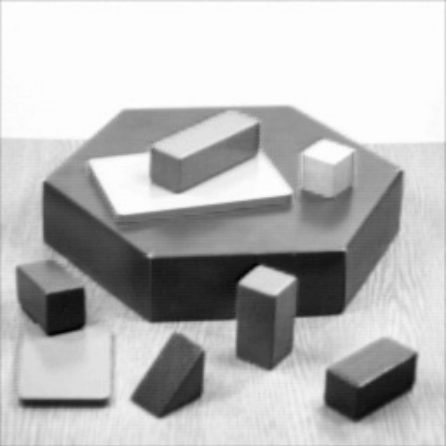
\includegraphics[width=1\linewidth]{recursos/imagens/image_seg/o1.png}
        \caption{Imagem original.}
        \label{segment:fig:7.1}
    \end{subfigure}%
    ~ 
    \begin{subfigure}[t]{0.45\textwidth}
        \centering
        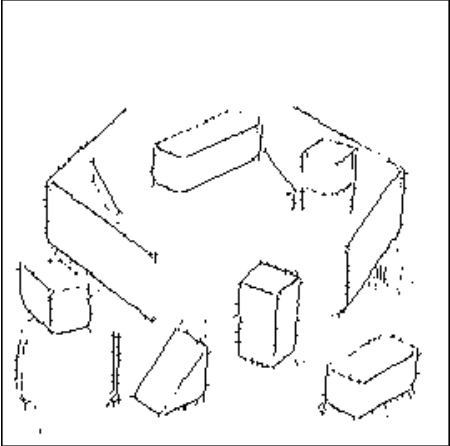
\includegraphics[width=1\linewidth]{recursos/imagens/image_seg/o2.png}
        \caption{Imagem resultante de $G_x$.}
        \label{segment:fig:7.2}
    \end{subfigure}%
    ~ 
    
    \begin{subfigure}[t]{0.45\textwidth}
        \centering
        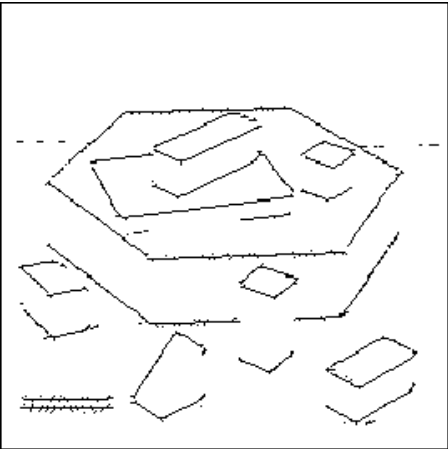
\includegraphics[width=1\linewidth]{recursos/imagens/image_seg/o3.png}
        \caption{Imagem resultante de $G_y$.}
        \label{segment:fig:7.3}
    \end{subfigure}
    ~
    \begin{subfigure}[t]{0.45\textwidth}
        \centering
        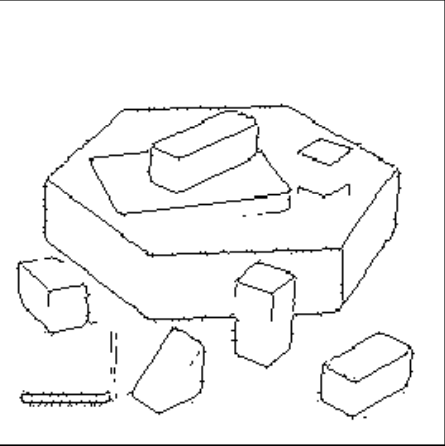
\includegraphics[width=1\linewidth]{recursos/imagens/image_seg/o4.png}
        \caption{Imagem de combinação entre $G_x$ e $G_y$.}
        \label{segment:fig:7.4}
    \end{subfigure}

    Fonte: \cite{pedrini2008analise}.
\end{figure}

Já em relação ao operador laplaciano, destaca-se que este faz uso de uma derivada segunda que pode ser representada a partir da Equação \ref{segment:eq:6}:

\begin{equation}
    \label{segment:eq:6}
    \bigtriangledown^2 f = \frac{\partial^2f}{\partial x^2} + \frac{\partial^2f}{\partial y^2},
\end{equation}
tendo que $f(x,y)$ é uma função bidimensional contínua e sendo recomendada para situações em que a imagem não tenha ruído e a posição da borda sejam mais relevantes \citep{Yuheng2017}. Isso se dá, visto que por contar com uma derivada de segunda ordem, torna-se muito sensível aos ruídos \citep{pedrini2008analise}.

Ainda sobre o operador laplaciano, pode se dizer que há uma necessidade de que o coeficiente do \textit{pixel} central resulte em um valor positivo e que os seus \textit{pixels} externos sejam negativos \citep{pedrini2008analise}. Assim, considerando uma matriz de vizinhança-8, pode-se exemplificar uma implementação do operador Laplaciano que considera as derivadas segundas em linhas e colunas tendo por base a matriz $H_1$ representada na Equação \ref{segment:eq:7}, resultando em aplicações como as visualizadas na Figura \ref{segment:fig:8}, sendo: 

\begin{equation}
    \label{segment:eq:7}
    H_1 = \begin{bmatrix}
     0 &  0 &  0 \\ 
    -1 &  2 & -1 \\ 
     0 &  0 &  0
    \end{bmatrix} +
    \begin{bmatrix}
     0 & -1 & 0 \\ 
     0 &  2 & 0 \\ 
     0 & -1 & 0 
    \end{bmatrix} =
    \begin{bmatrix}
     0 & -1 & 0 \\ 
    -1 &  4 & -1 \\ 
     0 & -1 & 0 
    \end{bmatrix}.
\end{equation}

\begin{figure}[H]
   \caption{Segmentação com operador Laplaciano.}
   \centering
   \label{segment:fig:8}
    \begin{subfigure}[t]{0.45\textwidth}
        \centering
        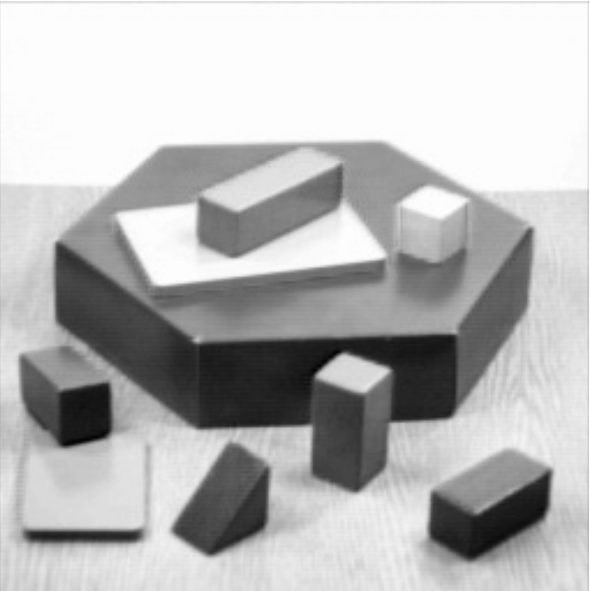
\includegraphics[width=1\linewidth]{recursos/imagens/image_seg/ol1.png}
        \caption{Imagem original.}
        \label{segment:fig:8.1}
    \end{subfigure}%
    ~ 
    \begin{subfigure}[t]{0.45\textwidth}
        \centering
        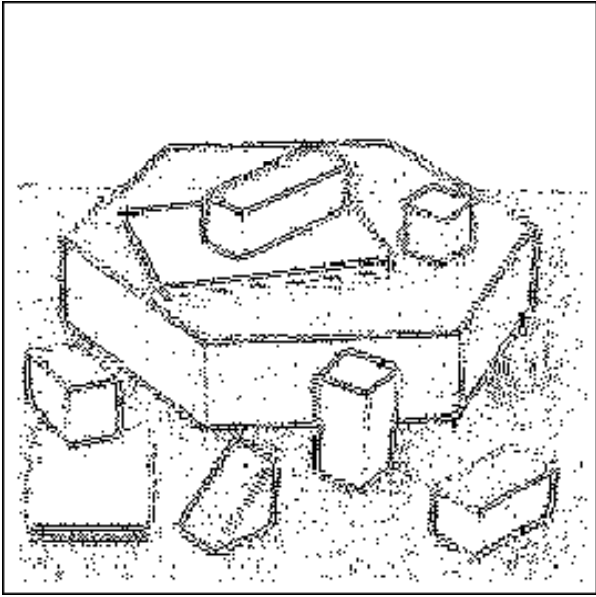
\includegraphics[width=1\linewidth]{recursos/imagens/image_seg/lp2.png}
        \caption{Mapa de bordas resultante.}
        \label{segment:fig:8.2}
    \end{subfigure}%

    Fonte: \cite{pedrini2008analise}.
\end{figure}

\subsubsection{Segmentação Baseada em Grafo}
\label{segment:graph}
A segmentação baseada em grafo é uma técnica robusta e versátil utilizada para dividir uma imagem em segmentos ou regiões. Esta abordagem consiste em modelar uma imagem como um grafo, onde cada nó representa um \textit{pixel} (ou um \textit{superpixel}, em certas implementações) e as arestas representam a relação entre os \textit{pixels} vizinhos. Tipicamente, essa relação é baseada na similaridade entre os nós, ou seja, \textit{pixels} com características visuais semelhantes, tais como intensidade, cor e textura, tendem a ser conectados por uma aresta \citep{Felzenszwalb2004EfficientSegmentation}.

A segmentação então envolve a subdivisão do grafo em subgrafos (ou regiões na imagem) que são internamente homogêneos e externamente heterogêneos. Existem diversos algoritmos para realizar essa tarefa, muitos deles baseados em técnicas de otimização de grafo, tais como o corte mínimo (\textit{min-cut}) e a expansão máxima de fluxo (\textit{max-flow}) \citep{Boykov2001FastCuts}.

Um algoritmo amplamente reconhecido na segmentação baseada em grafos é o algoritmo de Felzenszwalb e Huttenlocher \citep{Felzenszwalb2004EfficientSegmentation}, que integra-se com algoritmos de \textit{superpixels}. Este método aborda a segmentação como um problema de agrupamento hierárquico e emprega o critério de dissimilaridade, conhecido como "Evidência de Borda" (em inglês, \textit{Evidence for a Boundary}), para determinar a fusão ou separação de dois nós (ou segmentos). Matematicamente, esta condição é expressa pela Equação \ref{segment:eq:graph}:

\begin{equation}
    \label{segment:eq:graph}
    D(C_i, C_j) = \frac{|B_{ij}|}{\min(|C_i|,|C_j|)} \leq k,
\end{equation}
onde $D(C_i, C_j)$ é a dissimilaridade entre os segmentos $C_i$ e $C_j$, $|B_{ij}|$ representa a diferença de intensidade entre as bordas dos segmentos $C_i$ e $C_j$, $|C_i|$ e $|C_j|$ são os tamanhos dos segmentos $C_i$ e $C_j$, respectivamente, e $k$ é um limiar que determina o equilíbrio entre a evidência de borda e a expansão dos componentes. Esta equação assegura que $D(\cdot)$ seja um predicado que geralmente determina se a borda entre os componentes é significativa o suficiente para separá-los (quando a borda é evidente), ou se os componentes devem ser fundidos (quando a borda não é clara).

Embora o algoritmo produza segmentações de alta qualidade, a seleção adequada dos parâmetros pode representar um desafio.

O trabalho \cite{falcao2004image} traz uma inovação com a Transformada de Floresta de Imagens (IFT), uma metodologia que modela a imagem como um grafo, abrindo caminho para operações de processamento de imagens baseadas na identificação de caminhos de custo mínimo. Este procedimento, proposto por \cite{falcao2004image}, permite uma segmentação eficaz ao conectar cada \textit{pixel} a um caminho mínimo, derivado de várias sementes, destacando-se pela sua adaptabilidade e eficiência. A IFT apoia a versatilidade da segmentação baseada em grafo ao simplificar a análise de imagens, fornecendo uma abordagem unificada para a segmentação e análise de contorno.

\subsubsection{Segmentação \textit{Watershed}}
\label{segment:watershed}
O algoritmo \textit{watershed} (ou bacia hidrográfica, em português) é uma técnica amplamente utilizada para segmentação de imagens. Seu nome se baseia na divisão das superfícies topográficas \citep{pedrini2008analise}, onde os valores dos \textit{pixels} formam determinadas \quotes{montanhas} e uma variação de duas intensidades altas forma um \quotes{vale}. O algoritmo \textit{watershed} tem como desafio encontrar um limiar para preencher esses vales a partir dos mínimos regionais, formando bacias de retenção e destacando algumas \quotes{montanhas} que consistem em segmentos de linhas de contorno dos objetos da imagem \citep{pedrini2008analise, SealWatershed:Approach}. É possível visualizar a imagem original e a imagem segmentada por meio do algoritmo \textit{watershed} a partir da Figura \ref{segment:fig:watershed_1}.

\begin{figure}[H]
   \caption{Exemplos de segmentação com a aplicação de \textit{watershed}.}
   \centering
   \label{segment:fig:watershed_1}
    \begin{subfigure}[t]{0.5\textwidth}
        \centering
        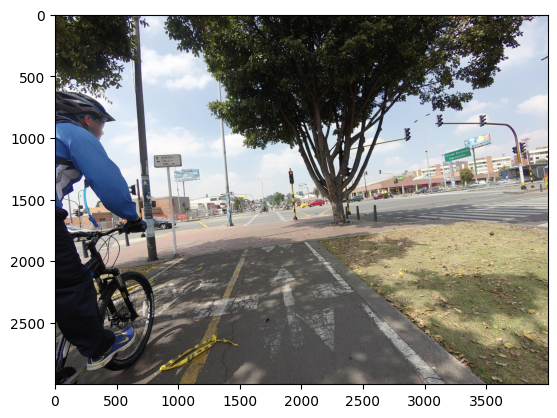
\includegraphics[width=1\linewidth]{recursos/imagens/image_seg/original_watershed.png}
        \caption{Imagem original.}
        \label{segment:fig:watershed_1.1}
    \end{subfigure}%
    ~ 

    \begin{subfigure}[t]{0.5\textwidth}
        \centering
        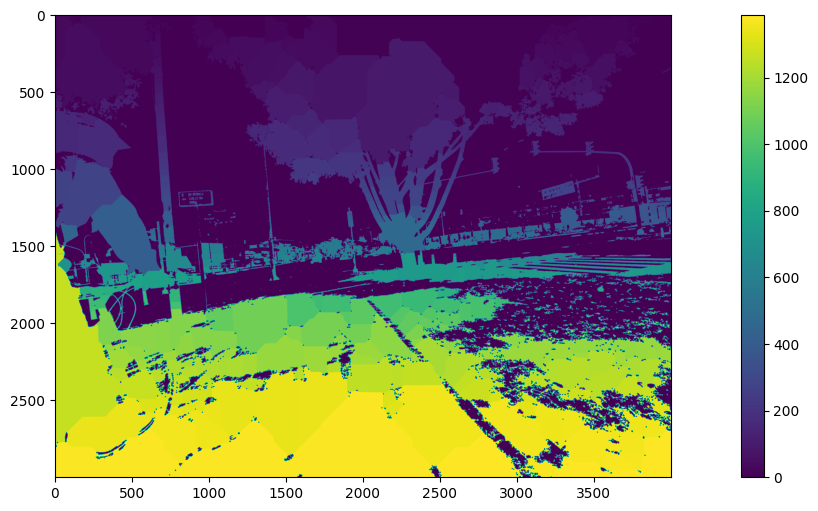
\includegraphics[width=1\linewidth]{recursos/imagens/image_seg/segmented_watershed.png}
        \caption{Imagem segmentada por \textit{watershed} com níveis do valor dos \textit{pixels} à direita.}
        \label{segment:fig:watershed_1.2}
    \end{subfigure}%
    ~

    Fonte: retirado e adaptado de \cite{Neuhold2017_ICCV}.
\end{figure}

Em resumo esse algoritmo pode ser realizado a partir do seguinte passo-a-passo:

\begin{enumerate}
    \item Transformação da imagem a ser segmentada em uma imagem de gradiente;
    \item Definição dos mínimos locais da imagem de gradiente como marcadores iniciais;
    \item Marcação dos \textit{pixels} vizinhos aos marcadores como pertencentes às suas respectivas bacias de retenção;
    \item Iterativamente, propagar as bacias de retenção até que elas se fundam em um \quotes{nível de água} comum;
    \item Extração das linhas de contorno das bacias de retenção para formar os objetos segmentados.
\end{enumerate}

Além disso, por meio da Figura \ref{segment:fig:watershed_2} é possível observar alguns resultados do processo de obtenção do resultado final, que é a imagem segmentada com a técnica \textit{watershed}.

\begin{figure}[H]
   \caption{Processo de segmentação \textit{watershed}.}
   \centering
   \label{segment:fig:watershed_2}
    \begin{subfigure}[t]{0.45\textwidth}
        \centering
        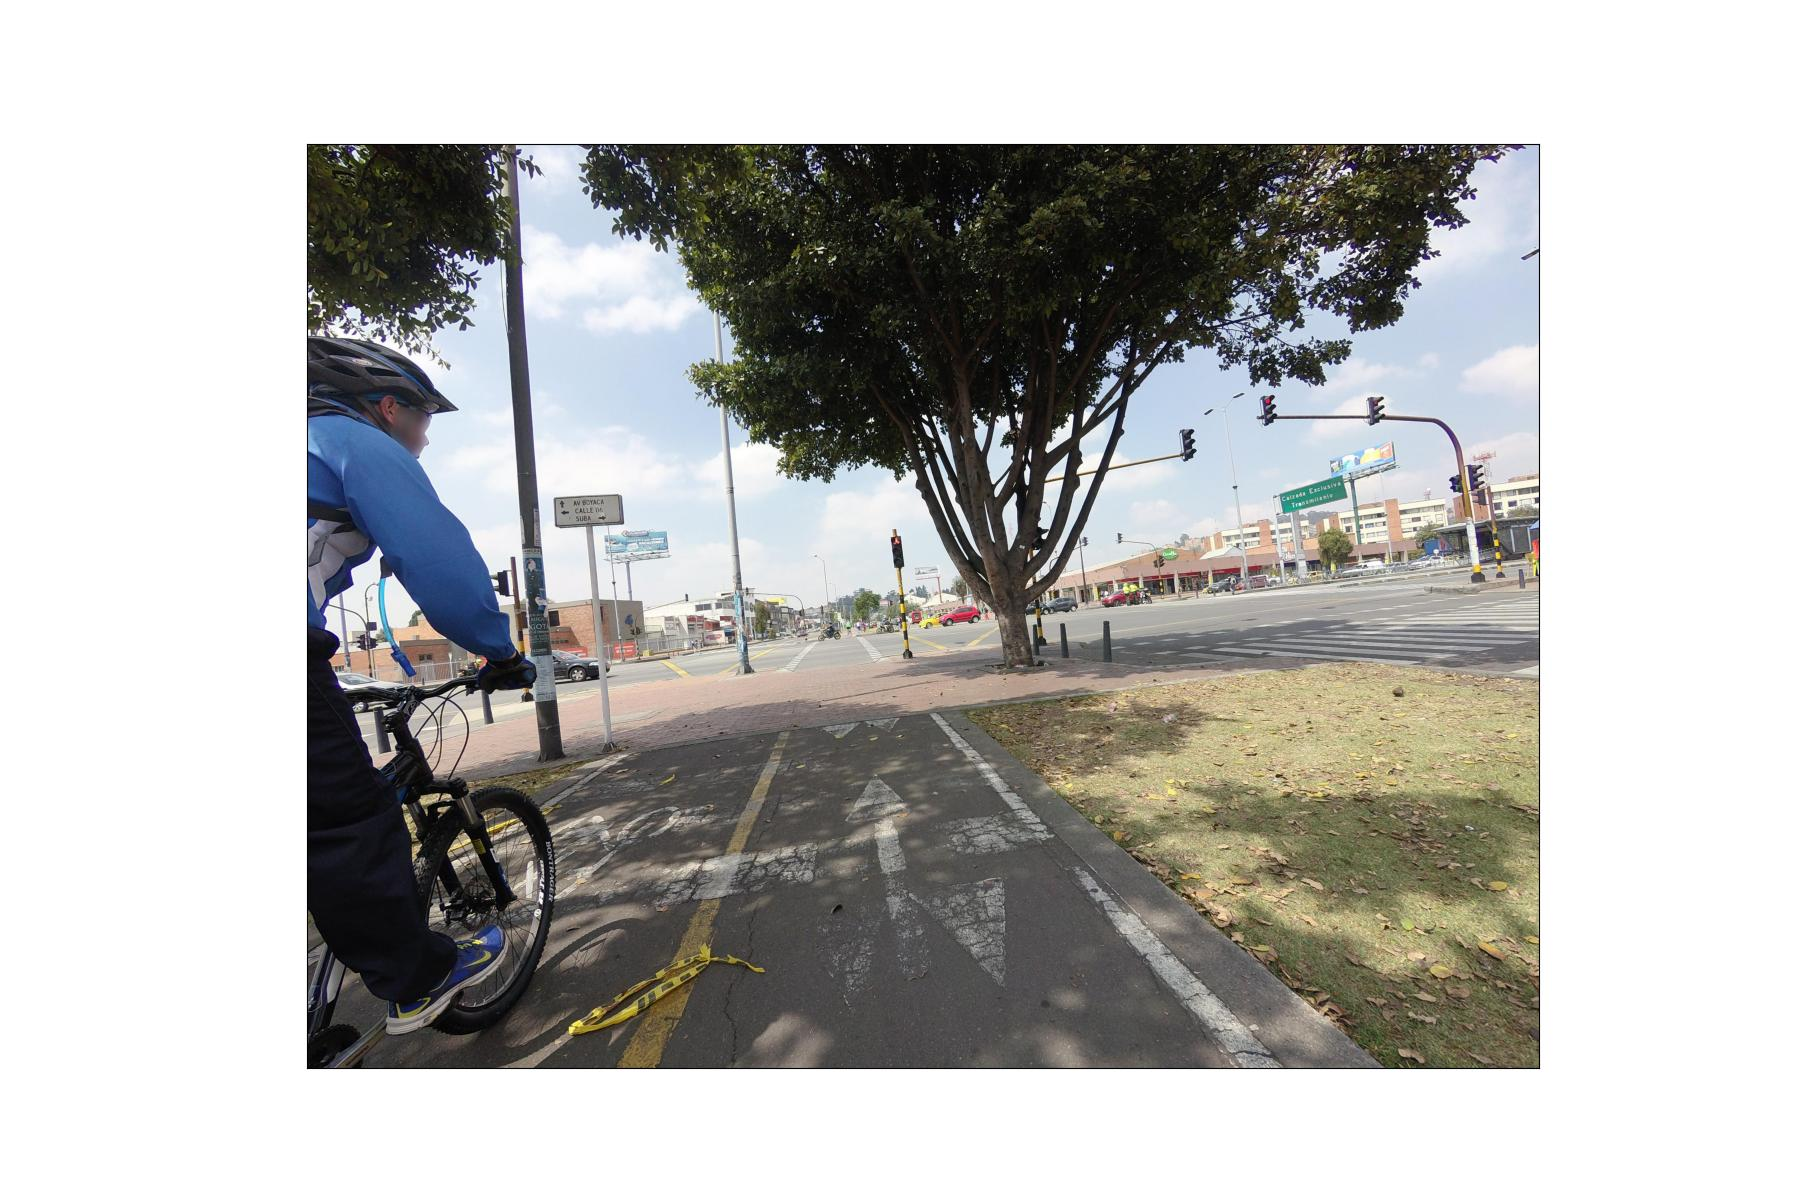
\includegraphics[width=1\linewidth]{recursos/imagens/image_seg/watershed0.jpg}
        \caption{Imagem original.}
        \label{segment:fig:watershed_2.1}
    \end{subfigure}%
    ~ 
    \begin{subfigure}[t]{0.45\textwidth}
        \centering
        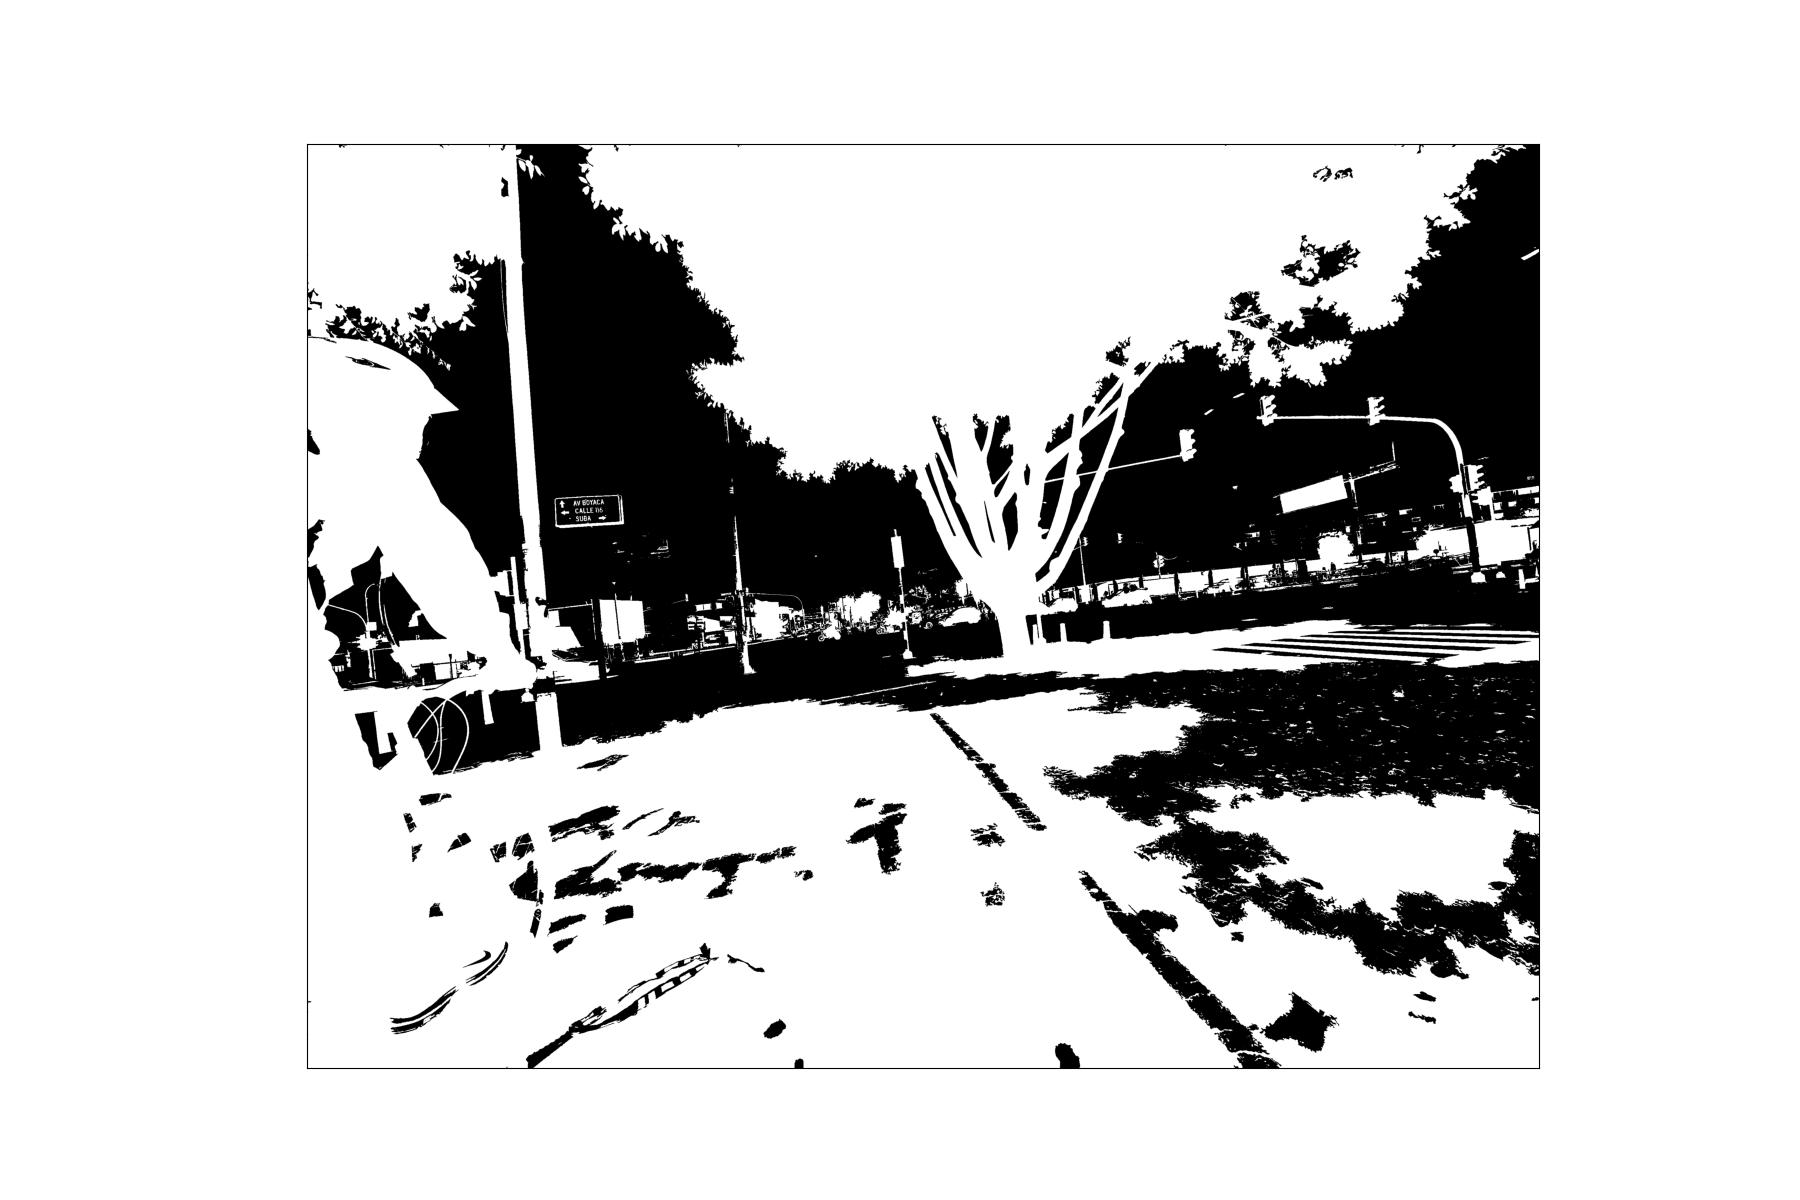
\includegraphics[width=1\linewidth]{recursos/imagens/image_seg/watershed1.jpg}
        \caption{Limiarização.}
        \label{segment:fig:watershed_2.2}
    \end{subfigure}%
    ~ 
    
    \begin{subfigure}[t]{0.45\textwidth}
        \centering
        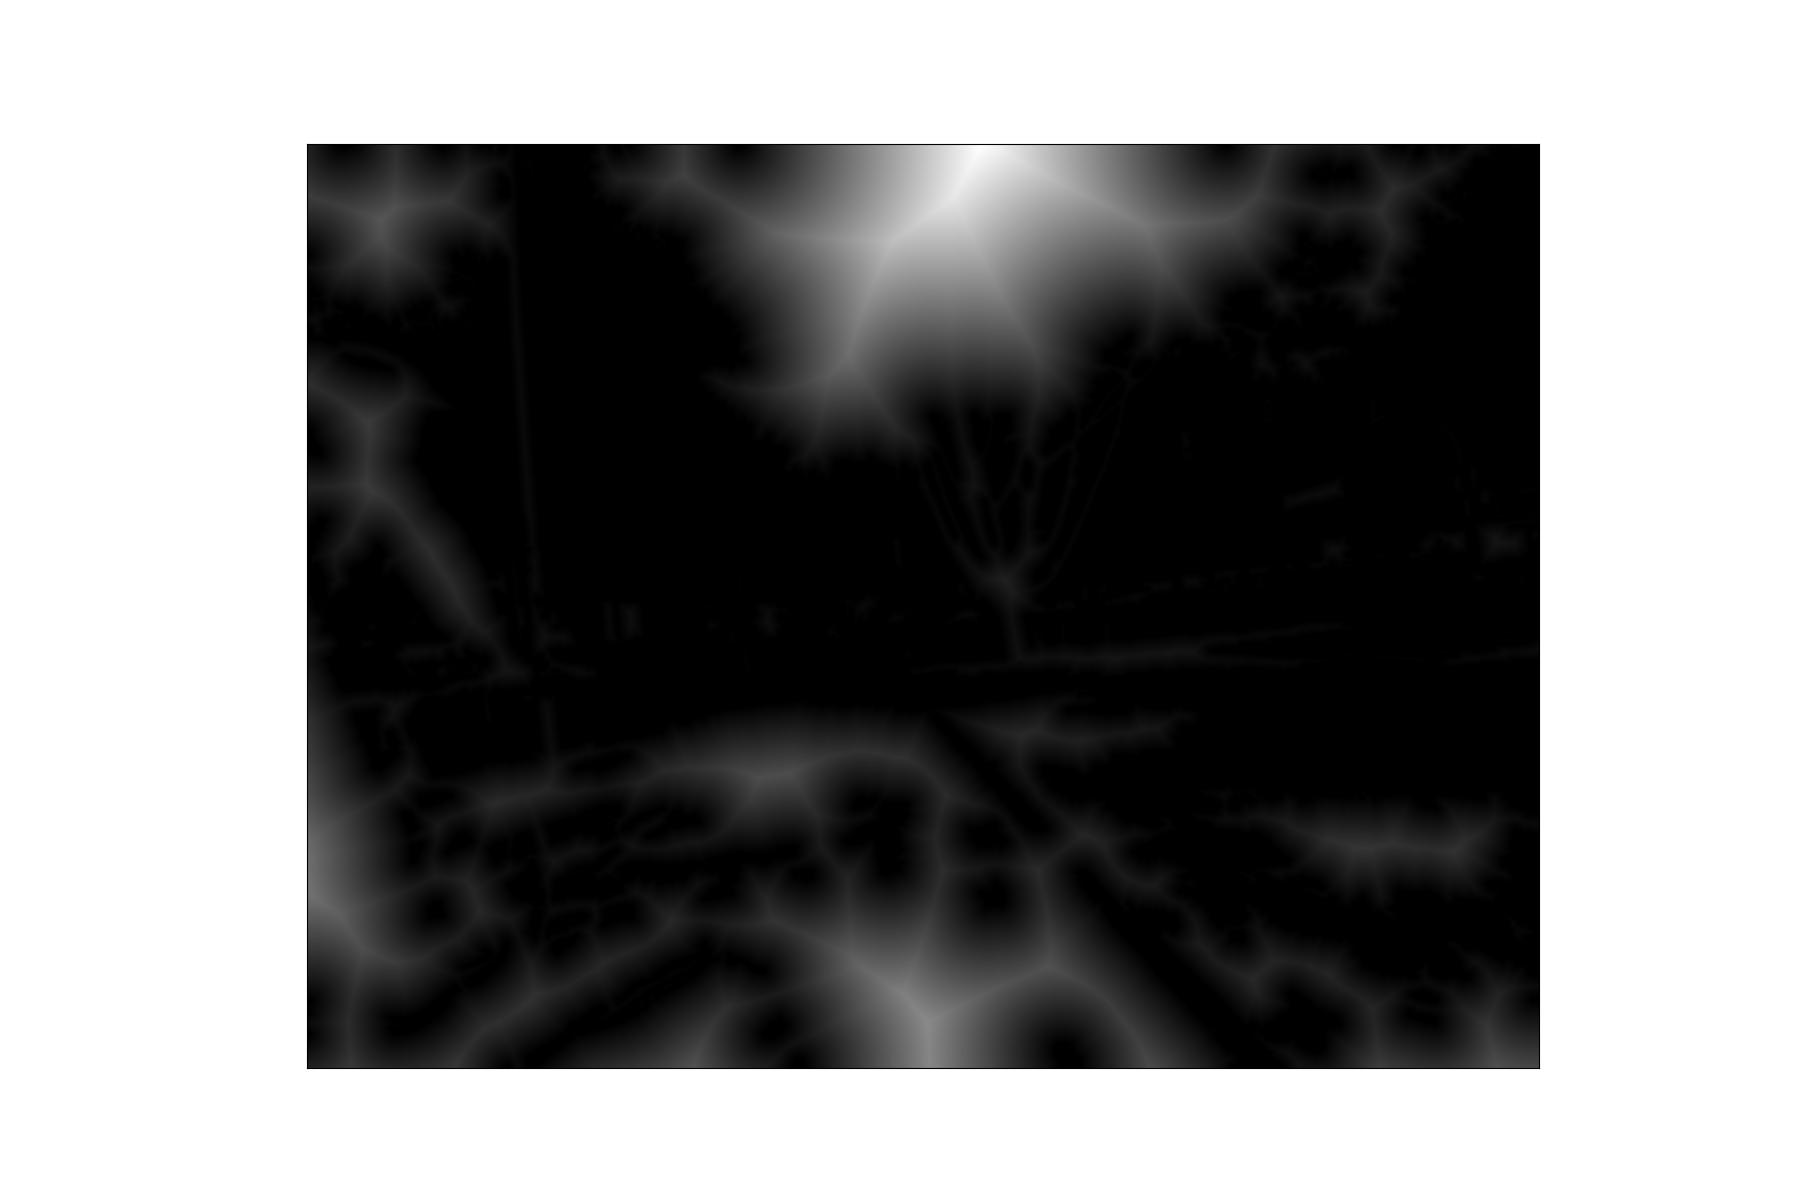
\includegraphics[width=1\linewidth]{recursos/imagens/image_seg/watershed2.jpg}
        \caption{Transformação das distâncias.}
        \label{segment:fig:watershed_2.3}
    \end{subfigure}
    ~
    \begin{subfigure}[t]{0.45\textwidth}
        \centering
        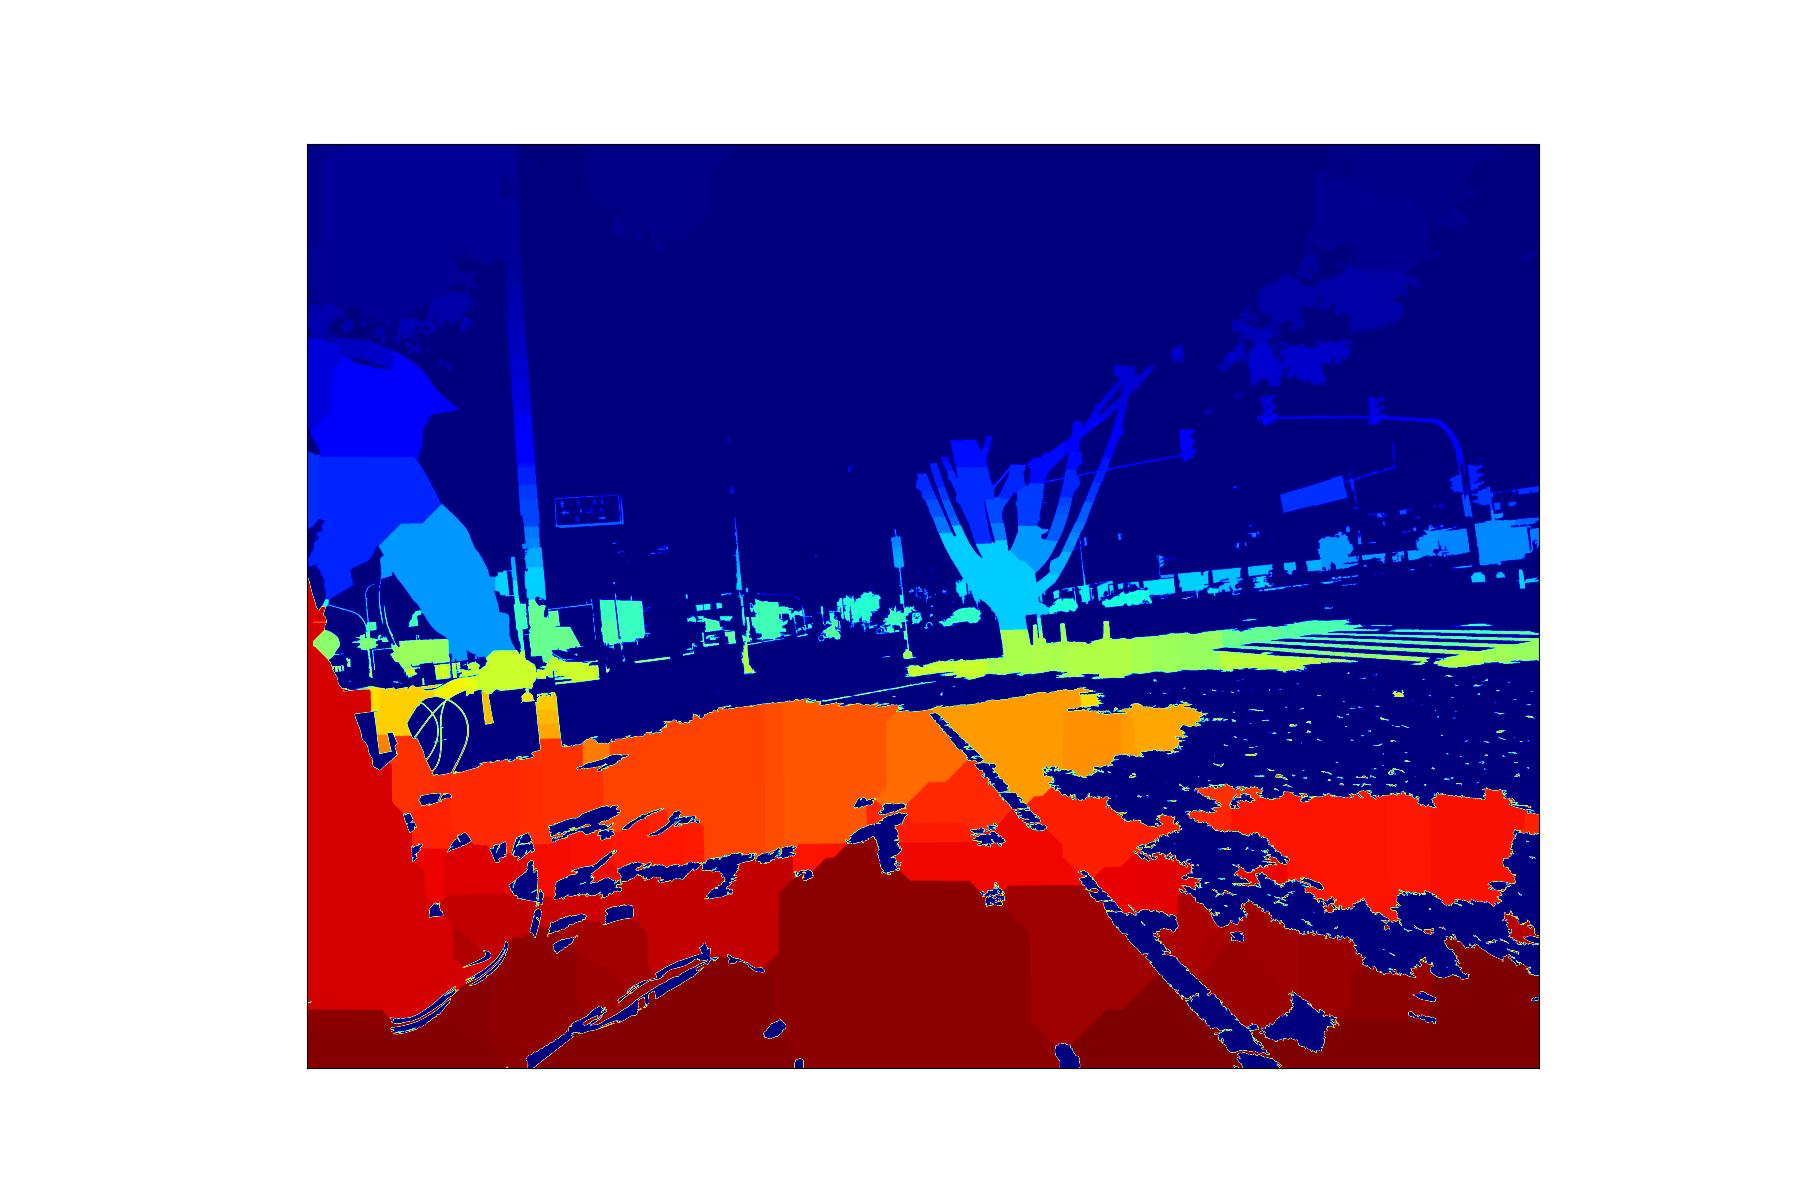
\includegraphics[width=1\linewidth]{recursos/imagens/image_seg/watershed3.jpg}
        \caption{Objetos segmentados.}
        \label{segment:fig:watershed_2.4}
    \end{subfigure}

    Fonte: retirado e adaptado de \cite{Neuhold2017_ICCV}.
\end{figure}


A deficiência desse algoritmo se dá pela sua sensibilidade em relação aos ruídos que são expressados por valores máximos ou mínimos na imagem, gerando assim, o aumento de regiões de segmentação \citep{pedrini2008analise}. Além disso, a descontinuidade das bordas de algumas imagens pode ocasionar em que algumas bacias cubram determinados contornos e impedindo a segmentação dos mesmos.

\subsubsection{Segmentação \textit{Livewire}}
\label{segment:livewire}
A segmentação \textit{livewire}, também conhecida como segmentação interativa ou segmentação assistida pelo usuário, é uma técnica na qual o usuário define um ponto inicial e um ponto final na imagem. A partir desses pontos, o processo da segmentação realiza automaticamente a identificação dos caminhos de menor custo entre o ponto inicial e final. Este custo geralmente é definido com base em características de borda, tal como o gradiente de intensidade, a direção de borda, e entre outros \citep{Falcao1997Paradigmas3D-Live-Wire}.

O método \textit{livewire}, proposto por \cite{Barrett1997InteractiveExtraction}, é um dos mais conhecidos para a segmentação interativa. A técnica emprega uma estrutura de grafo para representar a imagem, na qual cada \textit{pixel} é considerado como um nó e as arestas são definidas pelas distâncias euclidianas entre os \textit{pixels} vizinhos. O custo de cada aresta é determinado com base nas características da borda, onde:

\begin{itemize}
    \item $f_{gradiente}(i, j)$ é uma função de custo baseada no gradiente de intensidade dos \textit{pixels} em $i$ e $j$,
    \item $f_{direcao}(i, j)$ é uma função de custo baseada na direção de borda dos \textit{pixels} em $i$ e $j$,
    \item $f_{tamanho}(i, j)$ é uma função de custo baseada na distância euclidiana (ou comprimento) dos \textit{pixels} em $i$ e $j$.
\end{itemize}

Essas características são combinadas para formar o custo total de uma aresta na estrutura de grafo, como expresso matematicamente pela Equação \ref{segment:eq:livewire}:

\begin{equation}
    \label{segment:eq:livewire}
    c_{(i, j)} = f_{gradiente}(i, j) + f_{direcao}(i, j) + f_{tamanho}(i, j),
\end{equation}
onde $c_{(i, j)}$ é o custo total de uma aresta entre os nós $i$ e $j$. 

Essas funções de custo garantem que as bordas bem definidas na imagem realcem-se e que as bordas contínuas e mais longas tenham um custo menor, direcionando o caminho preferencial para estas.

Vale citar que geralmente, a técnica \textit{livewire} é muito eficiente em imagens médicas onde as bordas dos objetos de interesse são claras e consistentes. Contudo, ela pode ter desempenho insatisfatório em imagens com ruído, baixo contraste ou descontinuidade nas bordas \citep{Falcao1997Paradigmas3D-Live-Wire}.

\begin{figure}[H]
    \centering
    \caption{Exemplo da segmentação \textit{livewire} para extração dos contornos da imagem.}
    \label{segment:fig:livewire}
    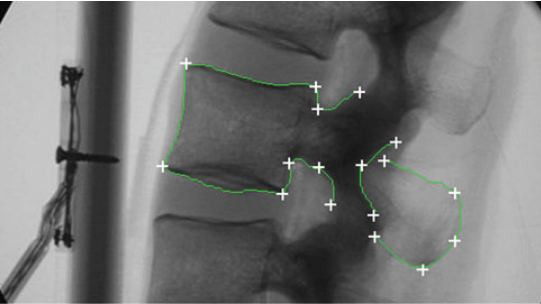
\includegraphics[width=0.8\linewidth]{recursos/imagens/image_seg/livewire.png}
    
    Fonte: retirado e adaptado de \cite{Zheng2011ScaledFluoroscopy}.
\end{figure}

Como ilustrado na Figura \ref{segment:fig:livewire}, o usuário pode iterativamente definir vários pontos iniciais e finais, e a técnica \textit{livewire} irá automaticamente conectar esses pontos formando a borda do objeto de interesse. Assim, a segmentação \textit{livewire} é um método semi-automático que combina a intuição do usuário com a eficiência da computação, fornecendo resultados de segmentação bastante precisos.

\subsubsection{Segmentação \textit{Superpixels}}
\label{segment:superpixel}
A noção de \textit{superpixels} foi introduzida por \cite{Ren2003LearningSegmentation} como uma forma de agrupar \textit{pixels} que compartilham características comuns, como cor, textura, e localização espacial, para formar uma unidade maior e mais coesa chamada de \textit{superpixel}. Essa abordagem de segmentação de imagens é frequentemente utilizada como um estágio preliminar para tarefas de compreensão de imagens e análise de cenas, pois pode reduzir significativamente a complexidade dos dados ao diminuir o número de unidades de processamento \citep{Achanta2012SLICMethods}.

Diversos algoritmos foram propostos para a geração de \textit{superpixels}, tais como: \textit{Simple Linear Iterative Clustering} (SLIC) \citep{Achanta2012SLICMethods}, \textit{Quick Shift} \citep{Vedaldi2008QuickSeeking}, Felzenszwalb \textit{Efficient Graph-Based Image Segmentation} \citep{Felzenszwalb2004EfficientSegmentation} e outros.

O algoritmo SLIC tem sido largamente utilizado devido à sua eficácia e eficiência. Esse método baseia-se no algoritmo K-means (que será discutido na Seção \ref{segment:group}) para clusterização de \textit{pixels}, mas, ao contrário do K-means, leva em conta tanto a cor (ou intensidade para imagens em escala de cinza) quanto a proximidade espacial dos \textit{pixels} \citep{Achanta2012SLICMethods}. Os \textit{superpixels} gerados com o algoritmo SLIC são compactos e pode-se controlar a quantidade desejada de \textit{superpixels}.

A Figura \ref{segment:fig:superpixel} ilustra a segmentação de \textit{superpixels} utilizando o algoritmo SLIC, \textit{Quick Shift} e Felzenszwalb em uma imagem. Cada segmento de \textit{superpixel} distinto na Figura \ref{segment:fig:superpixel.2} representa um separação de cor diferente. Como pode ser observado, os \textit{superpixels} aderem bem às bordas dos objetos na cena, o que os torna uma unidade de processamento útil para várias tarefas de análise de imagem no campo de visão computacional. Além disso, reduzir a imagem aos \textit{superpixels} em alguns casos, pode permitir diminuir o tempo de processamento para regiões de interesse, sem perder muita informação relevante.

\begin{figure}[H]
   \caption{Exemplo da segmentação com \textit{superpixels}.}
   \centering
   \label{segment:fig:superpixel}
    \begin{subfigure}[t]{0.45\textwidth}
        \centering
        \includegraphics[width=1\linewidth]{recursos/imagens/image_seg/superpixel_original.png}
        \caption{Imagem original}
        \label{segment:fig:superpixel.1}
    \end{subfigure}%
    ~ 
    \begin{subfigure}[t]{0.45\textwidth}
        \centering
        \includegraphics[width=1\linewidth]{recursos/imagens/image_seg/slic.png}
        \caption{\textit{Superpixel} com SLIC.}
        \label{segment:fig:superpixel.2}
    \end{subfigure}%
    ~ 
    
    \begin{subfigure}[t]{0.45\textwidth}
        \centering
        \includegraphics[width=1\linewidth]{recursos/imagens/image_seg/quick.png}
        \caption{\textit{Superpixel} com \textit{Quick Shift}.}
        \label{segment:fig:superpixel.3}
    \end{subfigure}
    ~
    \begin{subfigure}[t]{0.45\textwidth}
        \centering
        \includegraphics[width=1\linewidth]{recursos/imagens/image_seg/fz.png}
        \caption{\textit{Superpixel} com Felzenszwalb.}
        \label{segment:fig:superpixel.4}
    \end{subfigure}
    
    Fonte: retirado e adaptado de \cite{Neuhold2017_ICCV}.
\end{figure}

\subsubsection{Segmentação Baseada em Agrupamentos}
\label{segment:group}

Como o nome propõe, as segmentações baseadas em agrupamentos na esfera de visão computacional e processamento de imagens são compostas pela agregação de \textit{pixels} que possuem características similares em determinado espaço de características \citep{Yuheng2017}. No entanto, a definição de agrupamento (ou \textit{clustering}) ainda não é concreta \citep{Yuheng2017}, haja vista que não é categorizada como segmentação por alguns autores, pois os agrupamentos são realizados no espaço de medidas, enquanto a segmentação ocorre no domínio espacial da imagem \citep{Haralick1985}.

Posto isso, destaca-se o uso do K-means \citep{macqueen1967some, bock2008origins}, o qual é um método não supervisionado que realiza agrupamento de dados de um \textit{dataset} de acordo com as suas similaridades e em quantidades desejadas ($k$). Ou seja, o algoritmo gera um ponto inicial randômico como centroide para um determinado \textit{cluster} e depois tenta atribuir os demais dados do \textit{dataset} aos \textit{clusters} de acordo com a sua proximidade. Para isso, o algoritmo usa a geometria (ou distância) euclidiana \citep{Mahmud2012}. Vale ressaltar que os pontos centroides são atualizados conforme as classificações que são feitas no algoritmo, e os mesmos param de atualizar quando o algoritmo cumpre seu objetivo de convergência, há poucas interações dos dados com diferentes \textit{clusters} ou através de um número fixo de iterações \citep{dunham2006data}, conforme representado no fluxograma da Figura \ref{segment:fig:6}, tendo que $n \in \mathbb{Z}$.

\begin{figure}[H]
    \centering
    \caption{Fluxograma do algoritmo K-means.}
    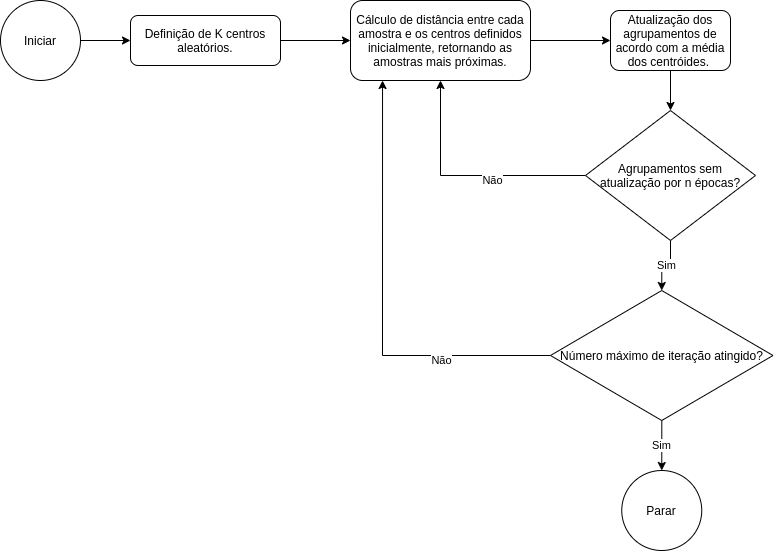
\includegraphics[width=1\linewidth]{recursos/imagens/image_seg/kmeans.png}
    \label{segment:fig:6}

    Fonte: do próprio autor.
\end{figure}

Na Figura \ref{segment:fig:5}, é possível observar resultado do uso do algoritmo K-means para agrupar as regiões da imagem, tendo que foi definido um valor de $k = 3$.

\begin{figure}[H]
   \caption{Segmentação com K-means.}
   \centering
   \label{segment:fig:5}
    \begin{subfigure}[t]{0.45\textwidth}
        \centering
        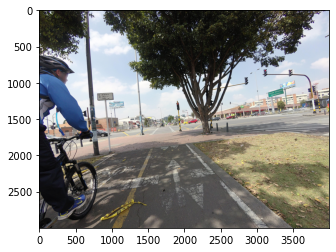
\includegraphics[width=1\linewidth]{recursos/imagens/image_seg/i1.png}
        \caption{Imagem original.}
        \label{segment:fig:5.1}
    \end{subfigure}%
    ~ 
    \begin{subfigure}[t]{0.45\textwidth}
        \centering
        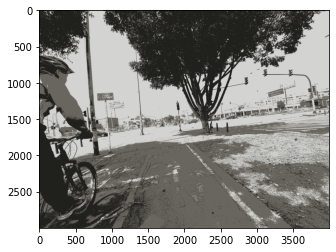
\includegraphics[width=1\linewidth]{recursos/imagens/image_seg/i2.png}
        \caption{Segmentação com $k = 3$.}
        \label{segment:fig:5.2}
    \end{subfigure}%

    Fonte: retirado e adaptado de \cite{Neuhold2017_ICCV}.
\end{figure}

\subsubsection{Segmentação com Redes Neurais}
\label{segment:neural}

A segmentação de imagens por meio de redes neurais (Capítulo \ref{deep}) ou redes convolucionais (Capítulo \ref{cnn}), é frequentemente associada à área de detecção de objetos devido à capacidade de demarcação e ao uso de caixas delimitadoras (em inglês, \textit{bounding boxes}) \citep{Ghosh2019}. No entanto, é importante salientar que, para as segmentações de imagens, as arquiteturas CNNs são amplamente utilizadas \citep{Goncalves2021}. Essas redes conseguem extrair as características mais relevantes de uma imagem e organizá-las, sendo eficazes não apenas em tarefas de detecção, localização e rastreamento de objetos, mas também na segmentação de imagens \citep{Ghosh2019}.

Um método mais recente que aborda essa tarefa e segue essa linha de raciocínio será detalhado no Capítulo \ref{semantic}, que trata das segmentações semânticas.

\subsection{Considerações Finais do Capítulo}
\label{segment:conclusion}

Na Tabela \ref{segment:table:1}, é possível visualizar as técnicas comentadas no decorrer do capítulo, assim como uma breve descrição de seus usos, suas vantagens e desvantagens.

\begin{landscape}
    \begin{table}[p]
    \centering
    \caption{Comparação entre os métodos de segmentações tradicionais.}
    \label{segment:table:1}
    
    \resizebox{\linewidth}{!}{%
        \scriptsize
        \begin{tabularx}{\linewidth}{l|X|X|X}
        \textbf{Técnica}                    & \textbf{Descrição}                                                                                                                                                & \textbf{Vantagens}                                                                                                                                                                                                     & \textbf{Desvantagens}                                                                                                                                                                               \\ 
        \hline
        Segmentação Baseada em Regiões      & Concentra-se em encontrar e agrupar valores semelhantes sendo separados por um limiar.                                                                             & - Possui baixa complexidade e alto desempenho; \newline - Não requer pré-processamento; \newline - Recomendado para imagens com alto contraste entre fundo e objeto de interesse.                                       & - Omissão de detalhes quando não há um contraste significante.                                                                                                                                       \\ 
        \hline
        Segmentação por Bordas              & Realizado com base na detecção de descontinuidade, detectando bordas e definindo um limite do objeto.                                                               & - Recomendável para imagens com bons contrastes entre os objetos.                                                                                                                                                        & - Perda de detalhes para imagens com muitas bordas, ruidosas ou com baixo contraste entre os objetos.                                                                                                 \\ 
        \hline
        Segmentação Baseada em Agrupamentos & Divide os \textit{pixels} da imagem em k \textit{clusters} homogêneos e exclusivos obtendo, assim, as segmentações.                                                  & - Conceitos já estabelecidos; \newline - Recomendado para aplicações em tempo real; \newline - Bom desempenho para pequenos \textit{datasets}; \newline - Não precisa de tempo de treinamento.                          & - Pode demandar muito tempo para encontrar a minimização da função de custo; \newline - Não é adequado para agrupar \textit{clusters} não convexos.                                                  \\ 
        \hline
        Segmentação Baseada em Grafos       & Representa uma imagem como um grafo, onde cada nó é um \textit{pixel} e as arestas são a relação entre os \textit{pixels} vizinhos.                                 & - Robusto e preciso; \newline - Flexível com variados tipos de imagens; \newline - Compatibilidade com outros métodos de segmentação.                                                                             & - Parâmetros podem ser difíceis de determinar; \newline - Sensível aos parâmetros; \newline - Podem ocorrer segmentações em excesso; especialmente em imagens ruidosas.                               \\
        \hline
        Segmentação  \textit{Superpixel}    & Agrupa \textit{pixels} que compartilham características comuns para formar uma maior unidade coesa denominada \textit{superpixel}.                                  & - Reduz a complexidade dos dados; \newline - Adere bem às bordas do objeto; \newline - Maior velocidade de processamento.                                                                                                 & - Pode perder detalhes finos das imagens; \newline - Parâmetros podem ser difíceis de determinar.                                                                                                    \\
        \hline
        Segmentação \textit{Watershed}      & Trata a imagem como um relevo topográfico, inundando todas as depressões a partir dos mínimos locais.                                                              & - Recomendável para imagens com bordas claras e bem definidas; \newline - Baixo custo computacional.                                                                                                                     & - Sensível a ruídos; \newline - Pode produzir segmentos excessivos.                                                                                                                                   \\
        \hline
        Segmentação \textit{Livewire}       & Abordagem interativa que elege um caminho de menor custo entre dois pontos escolhidos pelo usuário.                                                                 & - Proporciona resultados de segmentação precisos; \newline - Aproveita a intuição do usuário; \newline - Eficiência em imagens médicas com bordas claras e consistentes.                                                   & - Desempenho insatisfatório em imagens com ruído, baixo contraste ou descontinuidade nas bordas.                                                                                                    \\
        \hline
        Segmentação com Redes Neurais       & Normalmente relacionada a algoritmos de aprendizado profundo e CNNs.                                                                                               & - Conceito já estabelecido; \newline - Abordagem simples e flexível.                                                                                                                                                    & - O treinamento do modelo pode consumir muito tempo e recursos.                                                                                                                                       \\
        \hline
        
        \end{tabularx}%
    }
    
    \vspace*{1 cm}
    Fonte: do próprio autor.
    \end{table}
\end{landscape}


Na Seção \ref{segment:segment}, abordamos os algoritmos comumente utilizados para segmentações, indo desde técnicas mais simples, como o método de \textit{threshold segmentation} (Seção \ref{segment:region}), até abordagens de maior complexidade baseadas em redes neurais artificiais (Seção \ref{segment:neural}). Contudo, como discutido por \cite{Ghosh2019} e \cite{Minaee2021}, atualmente existem abordagens de segmentação que empregam \textit{deep learning} e apresentam excelentes desempenhos, sendo capazes de realizar segmentações de imagens e áreas de interesse em nível de \textit{pixel}. Uma dessas abordagens será explorada no próximo capítulo.
